\section{The One-Shot Phenomenon}
\label{sec:one-shot}

This section presents the experimental setup and results of One-Shot OPD. We investigate \textit{how much of full-data OPD's gain a single query recovers, and how robust that gain is}.

\begin{tcolorbox}[takeawaysbox]
\textbf{One query is enough to induce robust OPD gains.}
    A single query recovers most of the teacher--student gap across task domains and model families. The gain is insensitive to query difficulty, response length, and sampling temperature, and a query the student never solves is as effective as one it always solves.
\end{tcolorbox}

\subsection{Experimental Setup}
\label{sec:setup}

We establish one-shot OPD across math, code generation, instruction following, and agentic tool use for controlled analysis to test generality.

\paragraph{Models.}

\begin{table}[t]
\centering
\small
\caption{
Student--teacher pairs used in our experiments.
}
\label{tab:full}
\setlength{\tabcolsep}{5pt}
\renewcommand{\arraystretch}{1.12}
\begin{tabularx}{\textwidth}{@{}lXX@{}}
\toprule
\textbf{Setting} & \textbf{Student} & \textbf{Teacher} \\
\midrule

\multirow{3}{*}{Mathematical reasoning}
& DeepSeek-R1-Distill-Qwen-1.5B\newline
{\footnotesize (R1-Distill-1.5B)}
& JustRL-DeepSeek-1.5B\newline
{\footnotesize (JustRL-1.5B)} \\

& Llama-3.2-3B-Instruct\newline
{\footnotesize (Llama-3B-It)}
& GT-Llama-3.2-3B-Instruct-MATH\newline
{\footnotesize (GT-Llama-3B-Math)} \\

& OLMo-3-7B-Instruct-DPO\newline
{\footnotesize (OLMo-7B-It-DPO)}
& OLMo-3-7B-Instruct\newline
{\footnotesize (OLMo-7B-It)} \\

\midrule

Code generation
& DeepSeek-R1-Distill-Qwen-1.5B\newline
{\footnotesize (R1-Distill-1.5B)}
& Nemotron-Research-Reasoning-Qwen-1.5B-v2-RLVE\newline
{\footnotesize (Nemotron-1.5B)} \\

Instruction following
& DeepSeek-R1-Distill-Qwen-1.5B\newline
{\footnotesize (R1-Distill-1.5B)}
& UltraData-IF-1.5B \\

Agentic tool use
& Qwen2.5-Coder-1.5B-Instruct\newline
{\footnotesize (Qwen-Coder-1.5B)}
& Hammer2.1-1.5b\newline
{\footnotesize (Hammer-1.5B)} \\

\bottomrule
\end{tabularx}
\end{table}

For each domain, we pair a student with a post-trained teacher from the same family. Table~\ref{tab:full} lists the full identifiers and the short names used throughout. Math, code generation, and instruction following share the student R1-Distill-1.5B \citep{deepseekai2025deepseekr1incentivizingreasoningcapability}, whose teachers are, respectively, JustRL-1.5B \citep{he2025justrl}, Nemotron-1.5B \citep{zeng2025rlve}, and an instruction-following variant we post-train from the same student (Appendix~\ref{app:IF-setup}). For agentic tool use, the student is Qwen-Coder-1.5B \citep{hui2024qwen2} and the teacher is Hammer-1.5B \citep{lin2024hammer}. To test whether the phenomenon is specific to Qwen-based pairs, we add two mathematical-reasoning pairs from other families: Llama-3B-It \citep{grattafiori2024llama} with GT-Llama-3B-Math \citep{zhang2025co}, and OLMo-7B-It-DPO with OLMo-7B-It \citep{olmo2025olmo}.

\paragraph{Datasets.}
The domain-specific training sets comprise DAPO-Math-17K \citep{yu2026dapo} for mathematical reasoning, Open-R1 Codeforces \citep{penedo2025codeforces} for code generation, a sampled subset of UltraData-SFT-2605 \citep{ultradata-sft-2605} for instruction following, and xLAM-function-calling-60K \citep{liu2024apigen} for agentic tool use. For One-shot OPD in mathematics, we select three queries spanning easy, medium, and hard initial difficulty, scored by the student's pass rate over 8 rollouts before training (\(8/8\), \(4/8\), and \(0/8\), respectively). In each of the other domains, the one-shot query is sampled randomly from the corresponding training set. Appendix~\ref{app:model-data} details the dataset preprocessing and the selected one-shot queries.

\paragraph{Training.}
We implement OPD in \texttt{veRL} \citep{sheng2025hybridflow}.
The mathematical-reasoning runs of this section optimize the top-\(k\) advantage of Eq.~\ref{eq:topk-advantage} with \(k=16\); the code, instruction-following, and agentic runs optimize the sampled-token advantage of Eq.~\ref{eq:token-advantage}.
Every update uses a batch of $64$ rollouts. We use AdamW with a learning rate of $10^{-6}$, a rollout temperature of $1.0$, and a gradient clip norm of $1.0$; remaining hyperparameters are listed in Table~\ref{tab:opd-hyperparams}.


\paragraph{Evaluation.}
For math, we evaluate on MATH-500 \citep{hendrycksmath2021}, AMC 2023 \citep{li2024numinamath}, and AIME 2025 \citep{balunovic2026matharena}, sampling 16 responses per problem and reporting avg@16 accuracy.
For code generation, LiveCodeBench v6 (LCB v6) \citep{jain2025livecodebench} uses 3 sampled solutions per problem and reports avg@3 with the official execution-based evaluator.
For instruction following, Multi-IF \citep{he2024multi} evaluates three-turn conversations and reports the final-turn score averaged over its eight languages.
For agentic tool use, BFCL v3 \citep{patil2025bfcl} reports avg@8 over the evaluated subsets. And the response caps are \(31{,}744\) tokens
for mathematics, \(65{,}536\) for LCB v6, \(16{,}384\) per turn for Multi-IF, and \(4{,}096\) for BFCL v3. Unless stated otherwise, mathematics figures report validation accuracy macro-averaged over MATH-500, AMC 2023, and AIME 2025, and a dashed line marks the teacher.


\begin{figure}[t]
  \centering
  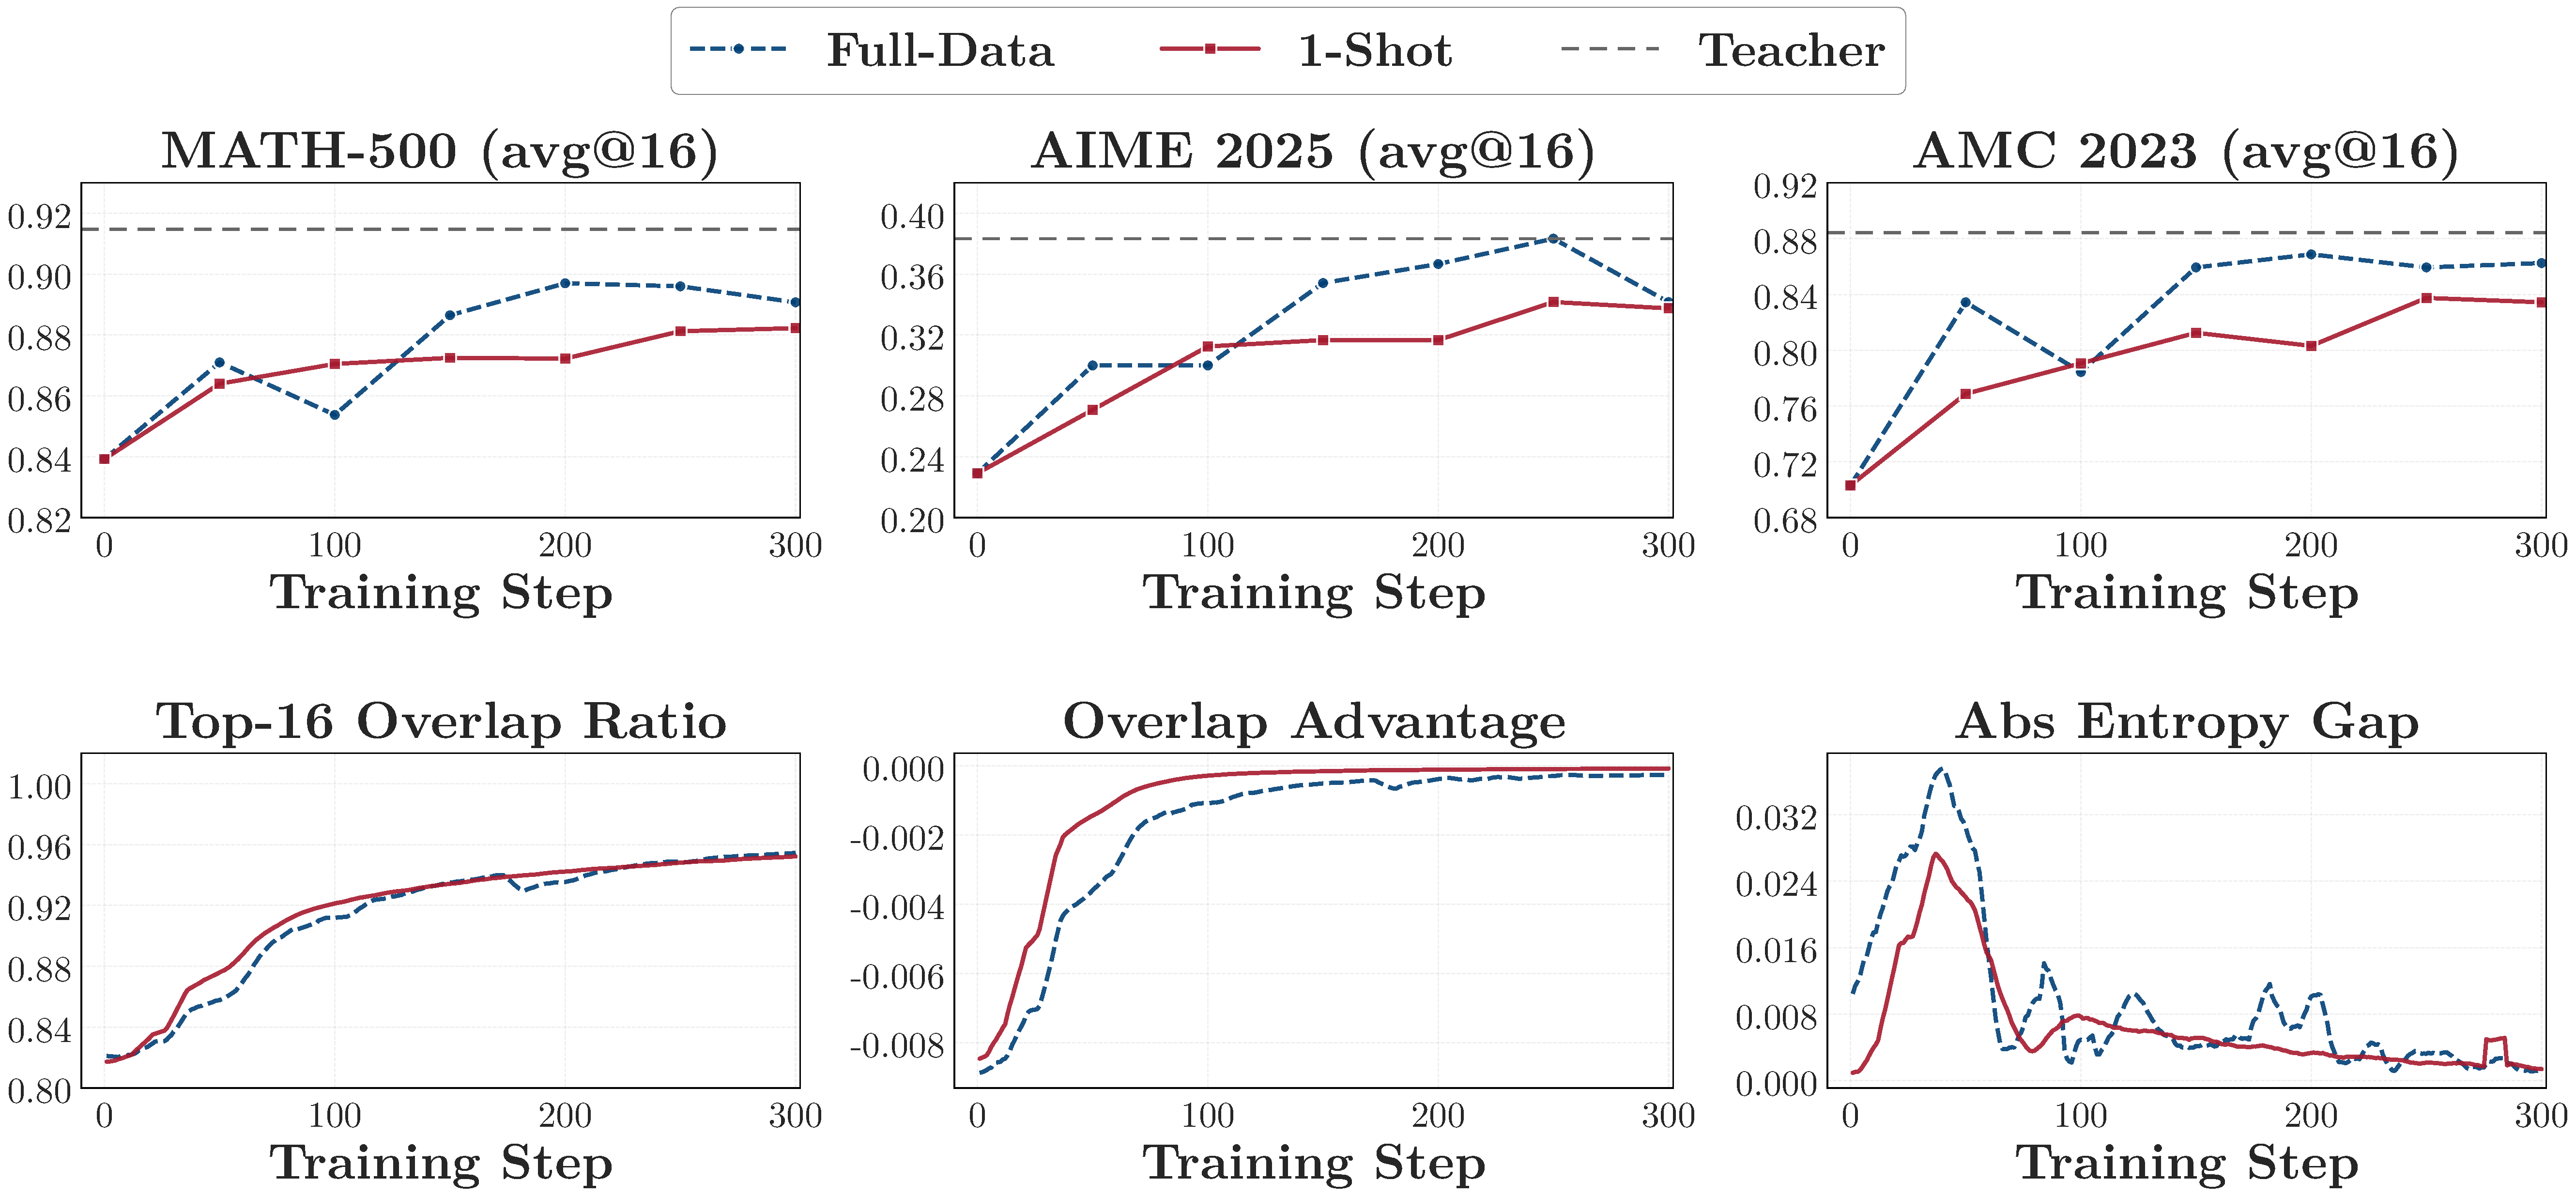
\includegraphics[width=\textwidth]{figures/3_oneshot_math300.pdf}
  \caption{Validation accuracy and Training dynamics of one-shot OPD on mathematical reasoning.}
  \label{fig:math_oneshot_dynamics}
\end{figure}

\begin{figure}[t]
  \centering
  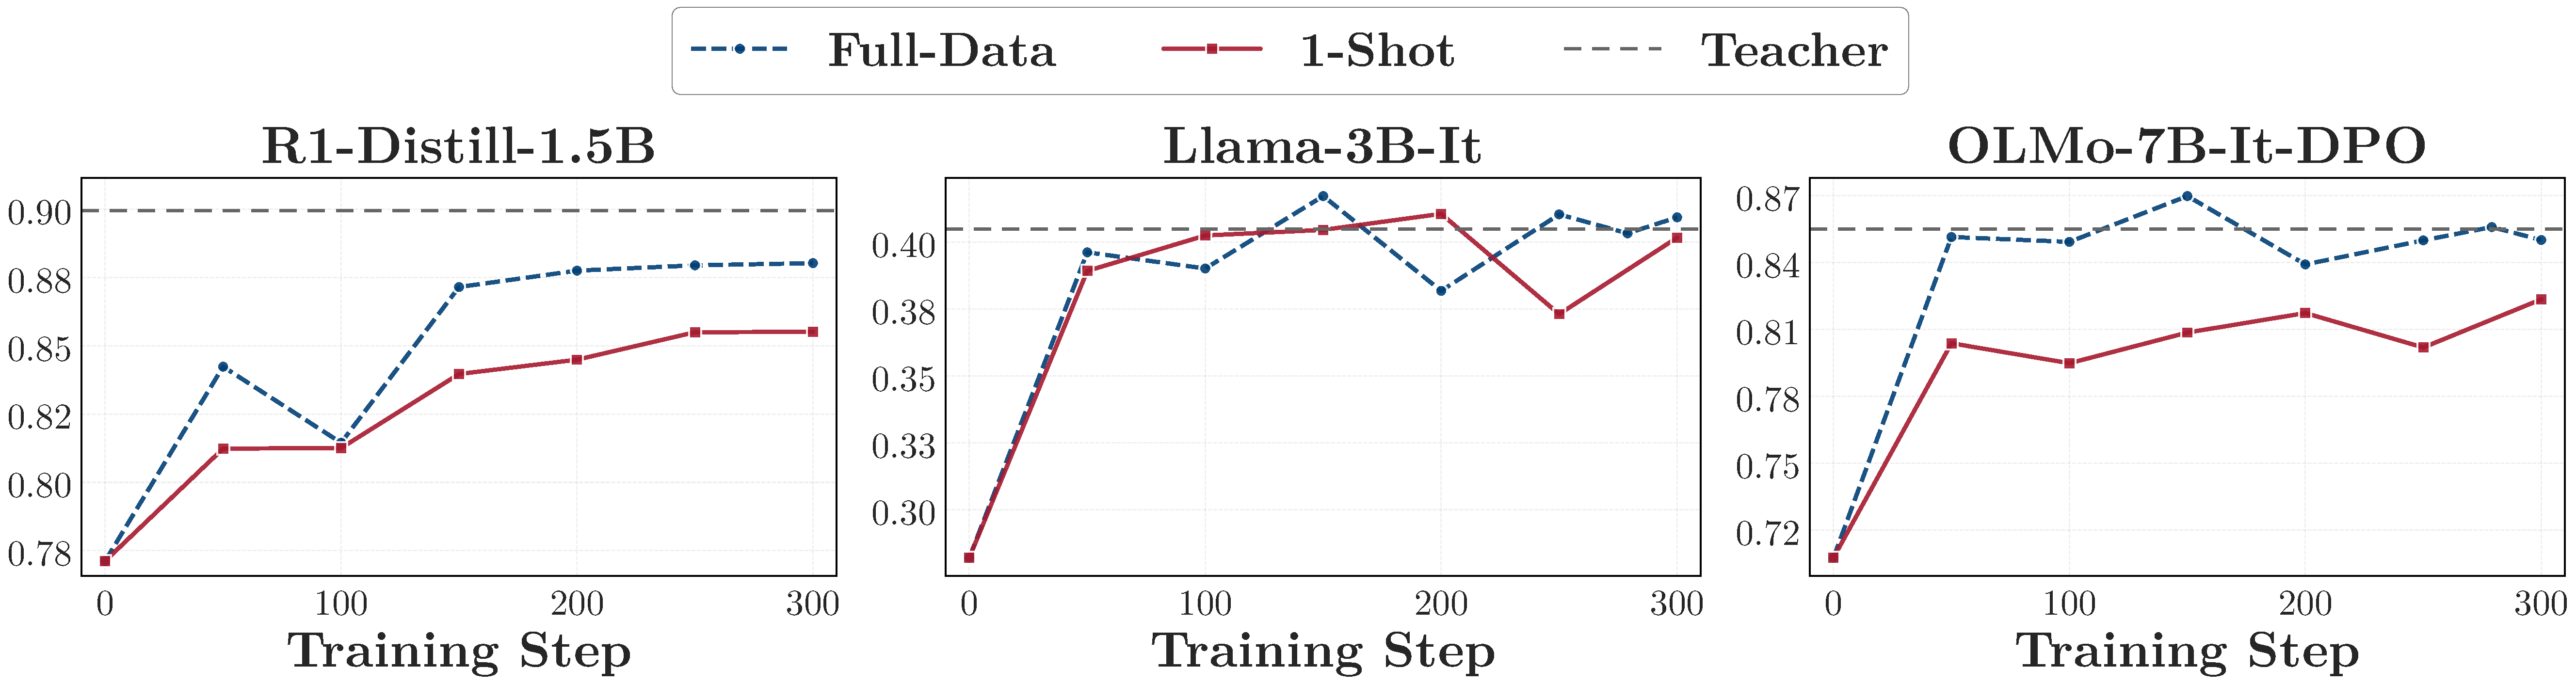
\includegraphics[width=\textwidth]{figures/3_cross_family.pdf}
  \caption{
  Validation accuracy of one-shot OPD across 3 student--teacher families, on mathematical reasoning averaged over MATH-500 and AMC 2023. AIME 2025 is excluded because the Llama pair scores near zero on it.
  }
  \label{fig:cross_family}
\end{figure}

\begin{figure}[t]
  \centering
  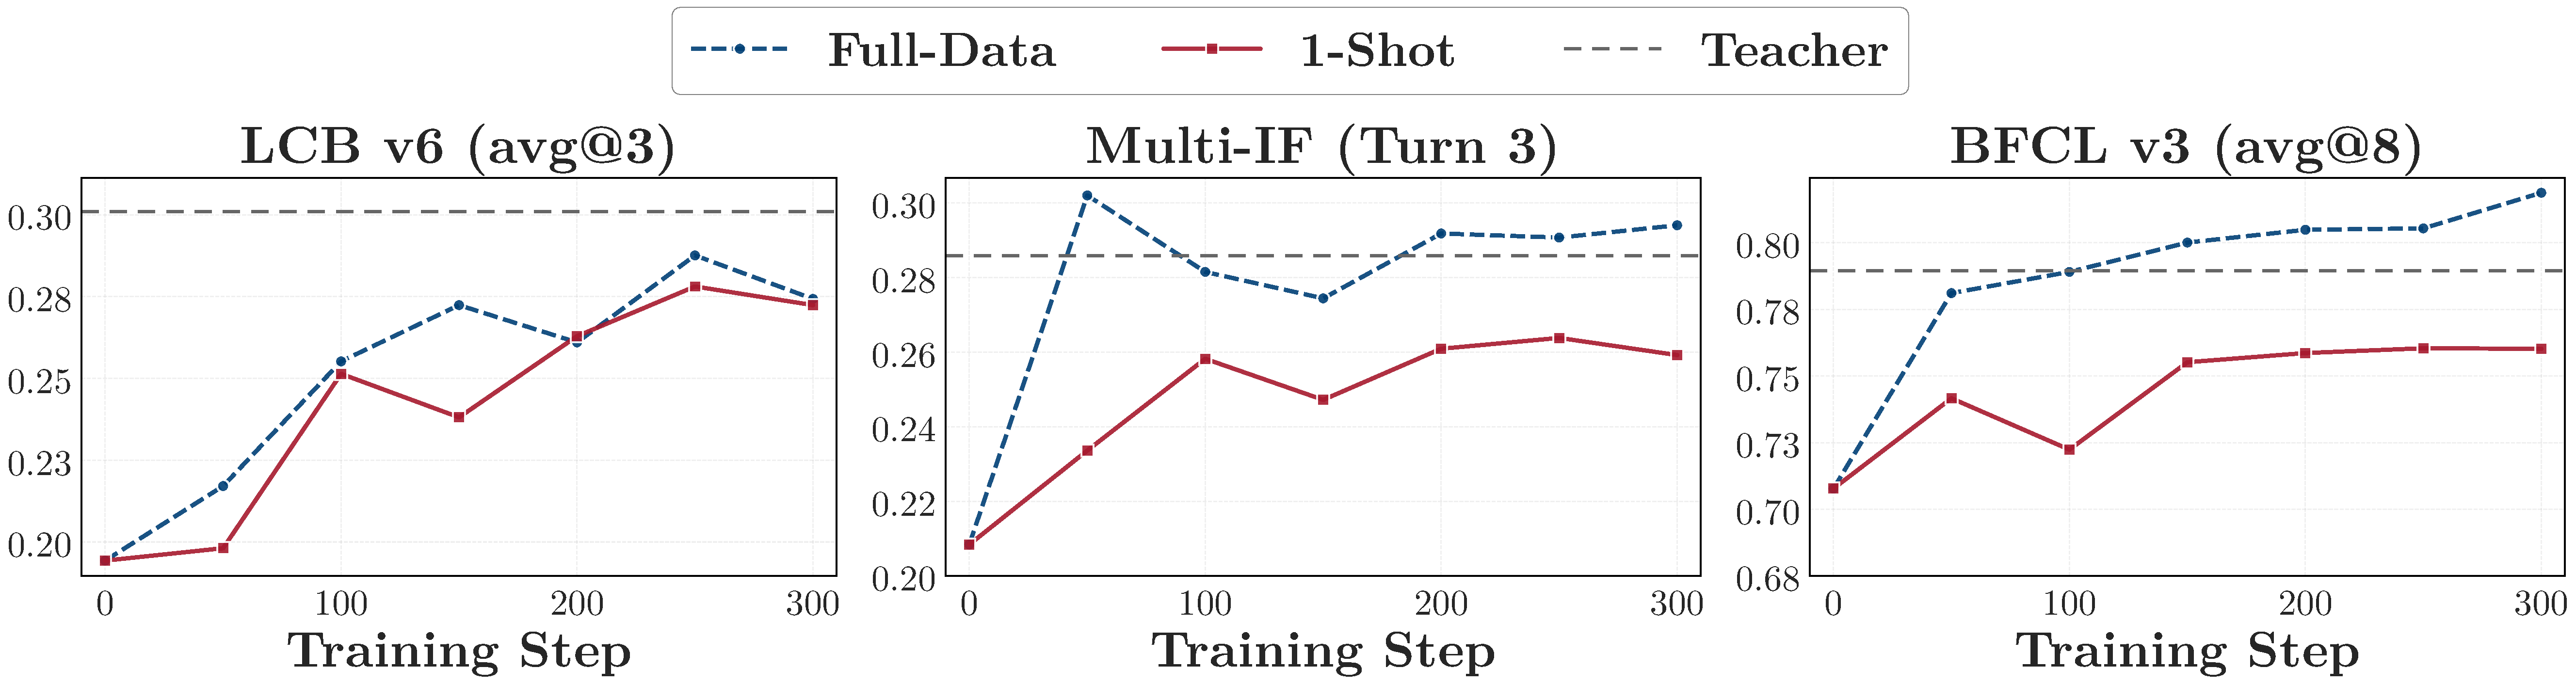
\includegraphics[width=\textwidth]{figures/3_cross_domain.pdf}
  \caption{
  Validation accuracy of one-shot OPD across three task domains.
  }
  \label{fig:cross_domain}
\end{figure}

\begin{figure}[t]
  \centering
  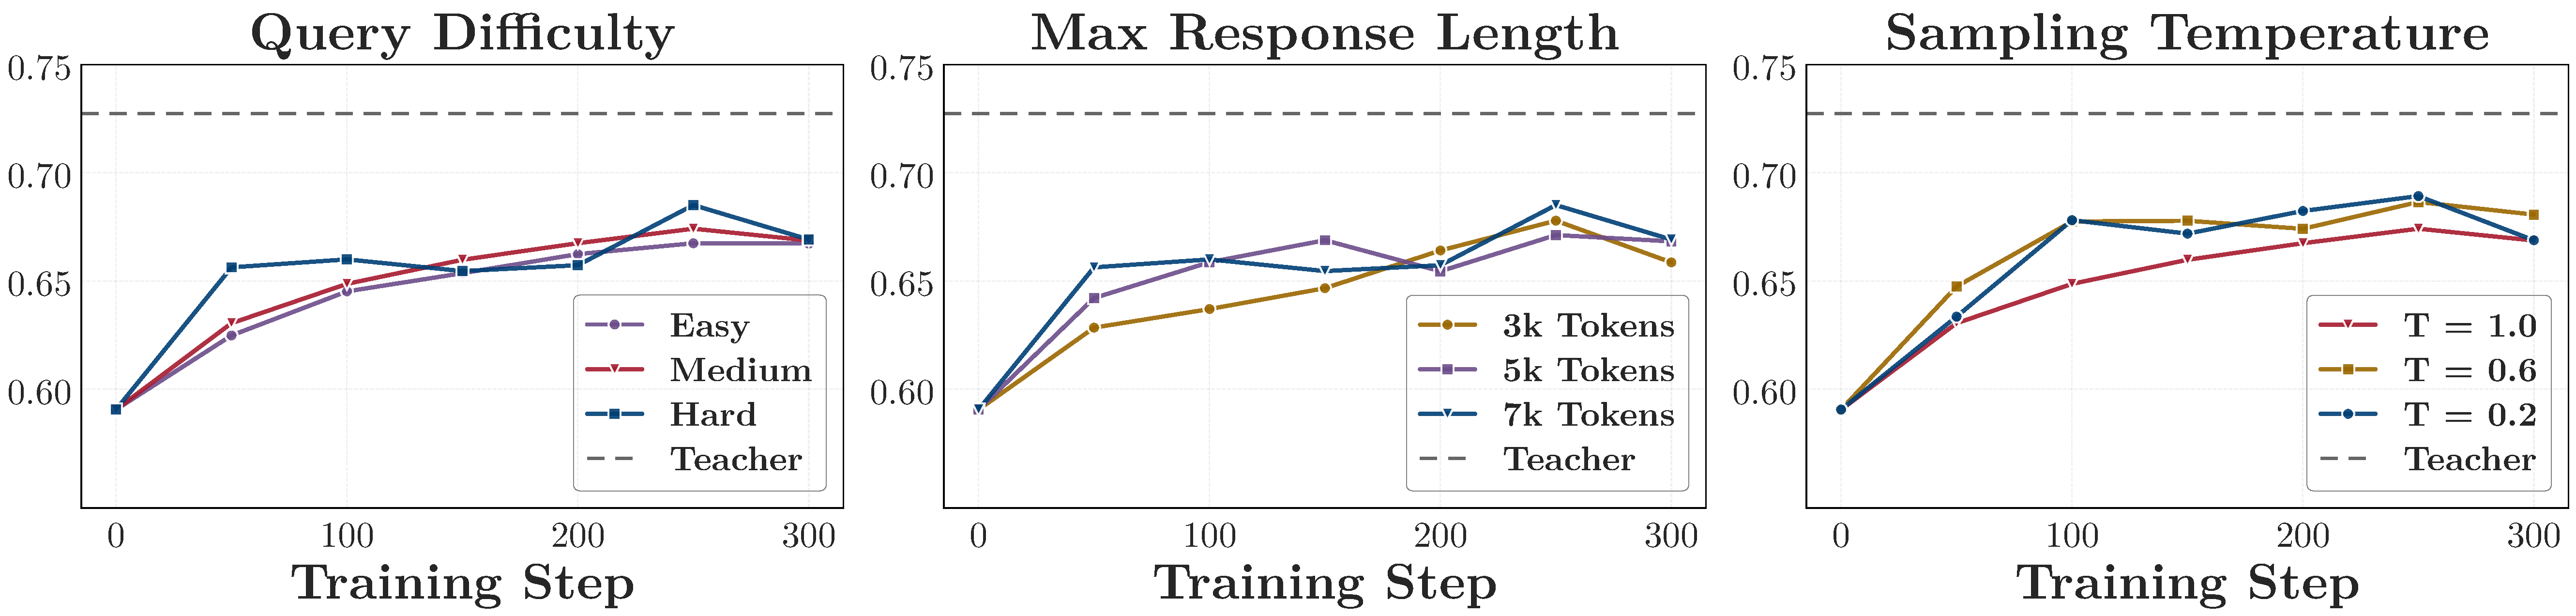
\includegraphics[width=\textwidth]{figures/3_ablations.pdf}
  \caption{
  Validation Accuracy of one-shot OPD under varying query difficulty, response-length cap on the hard query, and sampling temperature on the medium query.
  }
  \label{fig:probe_prompt}
\end{figure}


\subsection{Experimental Results}
% \subsection{A Single Query Recovers Most of Full-Data OPD's Gain Robustly}
\label{sec:finding-recovery}

\paragraph{One-shot OPD recovers most of full-data OPD's gain in mathematics.}

Figure~\ref{fig:math_oneshot_dynamics} shows that training on a single query improves accuracy on MATH-500, AIME 2025, and AMC 2023, approaching the full-data OPD on all three benchmarks. Averaged over them, one-shot OPD reaches \(68.5\) against \(69.8\) for full-data OPD, recovering \(69\%\) of the teacher--student gap and \(87\%\) of full-data OPD's gain at step 300. Beyond step \(300\) both curves stay within a band of about \(3\) points, and the recovered fraction ranges from \(62\%\) to \(89\%\) through step \(1000\), where one-shot OPD reaches \(68.4\) against \(72.1\) and recovers \(72\%\) of full-data OPD's gain (Figure~\ref{fig:teaser}). The training dynamics follow the same alignment process under both settings: the top-16 overlap ratio climbs to the full-data level, the overlap-token advantage approaches zero, and the absolute entropy gap nearly closes. Thus, even when all rollouts originate from a single query, OPD improves accuracy while progressively aligning the student distribution with the teacher on the visited states.


\paragraph{The one-shot effect is robust across families and task domains.}
\label{sec:one-shot-robust}
Figure~\ref{fig:cross_family} shows that one-shot OPD improves mathematical reasoning across all three student--teacher families. At the final checkpoint, the averaged scores increase from \(77.1\), \(28.2\), and \(70.8\) for the respective student baselines to \(85.5\), \(40.2\), and \(82.4\) for R1-Distill-1.5B, Llama-3B-It, and OLMo-7B-It-DPO. Figure~\ref{fig:cross_domain} further shows that the effect extends beyond mathematical reasoning: on code generation, instruction following, and agentic tool use, one-shot OPD recovers \(73\%\), \(66\%\), and \(64\%\) of the corresponding teacher--student gaps, respectively. Together, these results show that the one-shot effect is robust across both model families and task domains.


\paragraph{The one-shot effect is robust to query and rollout properties.}

We next examine whether one-shot OPD remains effective under varying query difficulty, response-length budgets, and rollout sampling temperature. As shown in Figure~\ref{fig:probe_prompt}, one-shot OPD works across easy, medium, and hard queries, even though the fraction of correct rollouts evolves very differently in the three settings (Appendix~\ref{app:training-accuracy}): the easy query is solved on nearly every step, the medium query becomes largely solvable during training, and the hard query is never solved. Tightening the response-length cap and lowering the rollout temperature both preserve the one-shot gain. Together, these results show that one-shot OPD is robust to query difficulty, response-length budget, and rollout sampling temperature.
